% This program can be redistributed and/or modified under the terms
% of the GNU Public License, version 3.
%
% Seth Brown, Ph.D.
% sethbrown@drbunsen.org
%
% Compiled with XeLaTeX
% Dependencies:
%   Fontin Sans font (http://www.exljbris.com/fontinsans.html)
%
\documentclass[xcolor={dvipsnames}]{beamer}

\usepackage[utf8]{inputenc}	%lettere accentate
\usepackage[italian]{babel}	%sillabazione italiana
\usepackage{amsmath}		%simboli matematici
\usepackage{amsfonts}		%font matematici
\usepackage{amssymb}		%altri simboli matematici
\usepackage{tikz}			%grafica
\usepackage{listings}		%codice\usepackage{graphicx} % graphics
\usepackage{epsfig} 		% eps graphics
\usepackage{hyperref} 		% urls
\usepackage{booktabs, caption} % table styling

% suppress navigation bar
\beamertemplatenavigationsymbolsempty

\mode<presentation>
{
	\usetheme{bunsen}
	\setbeamercovered{transparent}
	\setbeamertemplate{items}[circle]
}

% set fonts
\usepackage{fontspec}
\setsansfont{Fontin}
\setbeamerfont{frametitle}{size=\LARGE,series=\bfseries}

% color definitions
\definecolor{uipoppy}{RGB}{225, 64, 0}
\definecolor{uipaleblue}{RGB}{96,123,139}
\definecolor{uiblack}{RGB}{0, 0, 0}
\definecolor{back}{rgb}{0.93,0.93,0.97} 

% caption styling
\DeclareCaptionFont{uiblack}{\color{uiblack}}
\DeclareCaptionFont{uipoppy}{\color{uipoppy}}
\captionsetup{labelfont={uipoppy},textfont=uiblack}

% see the macros.tex file for definitions
% This program can be redistributed and/or modified under the terms
% of the GNU Public License, version 3.

% adds reference to bottom right of corner of a slide
\usepackage[absolute,overlay]{textpos} % text references in slide corners
\newcommand\textref[1]{%
  \begin{textblock*}{\paperwidth}(0pt,0.99\textheight)
  \raggedleft \tiny{\emph{#1}}\hspace{.5em}
  \end{textblock*}}

% for drawing circles around numbers
% ex. \circled{1} Add some text here.
\usepackage{tikz}
\newcommand*\circled[1]{\tikz[baseline=(char.base)]{
            \node[shape=circle,draw,inner sep=2pt] (char) {#1};}}


\lstset{ %
	backgroundcolor=\color{back},  	% choose the background color; you must add \usepackage{color} or \usepackage{xcolor}; should come as last argument
	basicstyle=\tiny,        		% the size of the fonts that are used for the code
	breakatwhitespace=false,        % sets if automatic breaks should only happen at whitespace
	breaklines=true,                % sets automatic line breaking
	captionpos=b,                   % sets the caption-position to bottom
	commentstyle=\color{gray},   	% comment style
	frame=single,	                % adds a frame around the code
	frameround=tttt					% round corner (use f instead t to edge corner)
	keepspaces=true,                % keeps spaces in text, useful for keeping indentation of code (possibly needs columns=flexible)
	keywordstyle=\color{blue},      % keyword style
	language=Python,               	% the language of the code
	numbers=none,                   % where to put the line-numbers; possible values are (none, left, right)
	numbersep=5pt,                  % how far the line-numbers are from the code
	numberstyle=\tiny\color{black}, % the style that is used for the line-numbers
	rulecolor=\color{black},        % if not set, the frame-color may be changed on line-breaks within not-black text (e.g. comments (green here))
	showspaces=false,               % show spaces everywhere adding particular underscores; it overrides 'showstringspaces'
	showstringspaces=false,         % underline spaces within strings only
	showtabs=false,                 % show tabs within strings adding particular underscores
	stepnumber=1,                   % the step between two line-numbers. If it's 1, each line will be numbered
	stringstyle=\color{OrangeRed},  % string literal style
	tabsize=2                   	% sets default tabsize to 2 spaces
}

\newcommand{\codice}[2]{\lstinputlisting[firstline=#1, lastline=#2]{code/PCA.py}}

\newcommand{\figcen}[2]{
	\begin{figure}
		\begin{center}
			\includegraphics[width=#1]{#2}
		\end{center}
	\end{figure}
}

% title slide definition
\title{Principal Component Analysis:\newline dalla teoria alla pratica}
\author{Marco Buracchi}
\institute{Università degli studi di Firenze}

\graphicspath{{img/}}
\logo{\includegraphics[scale=0.03]{logo.eps}}

\date{\today}

%--------------------------------------------------------------------
%                           Introduction
%--------------------------------------------------------------------

\begin{document}
	
	\setbeamertemplate{background}
	{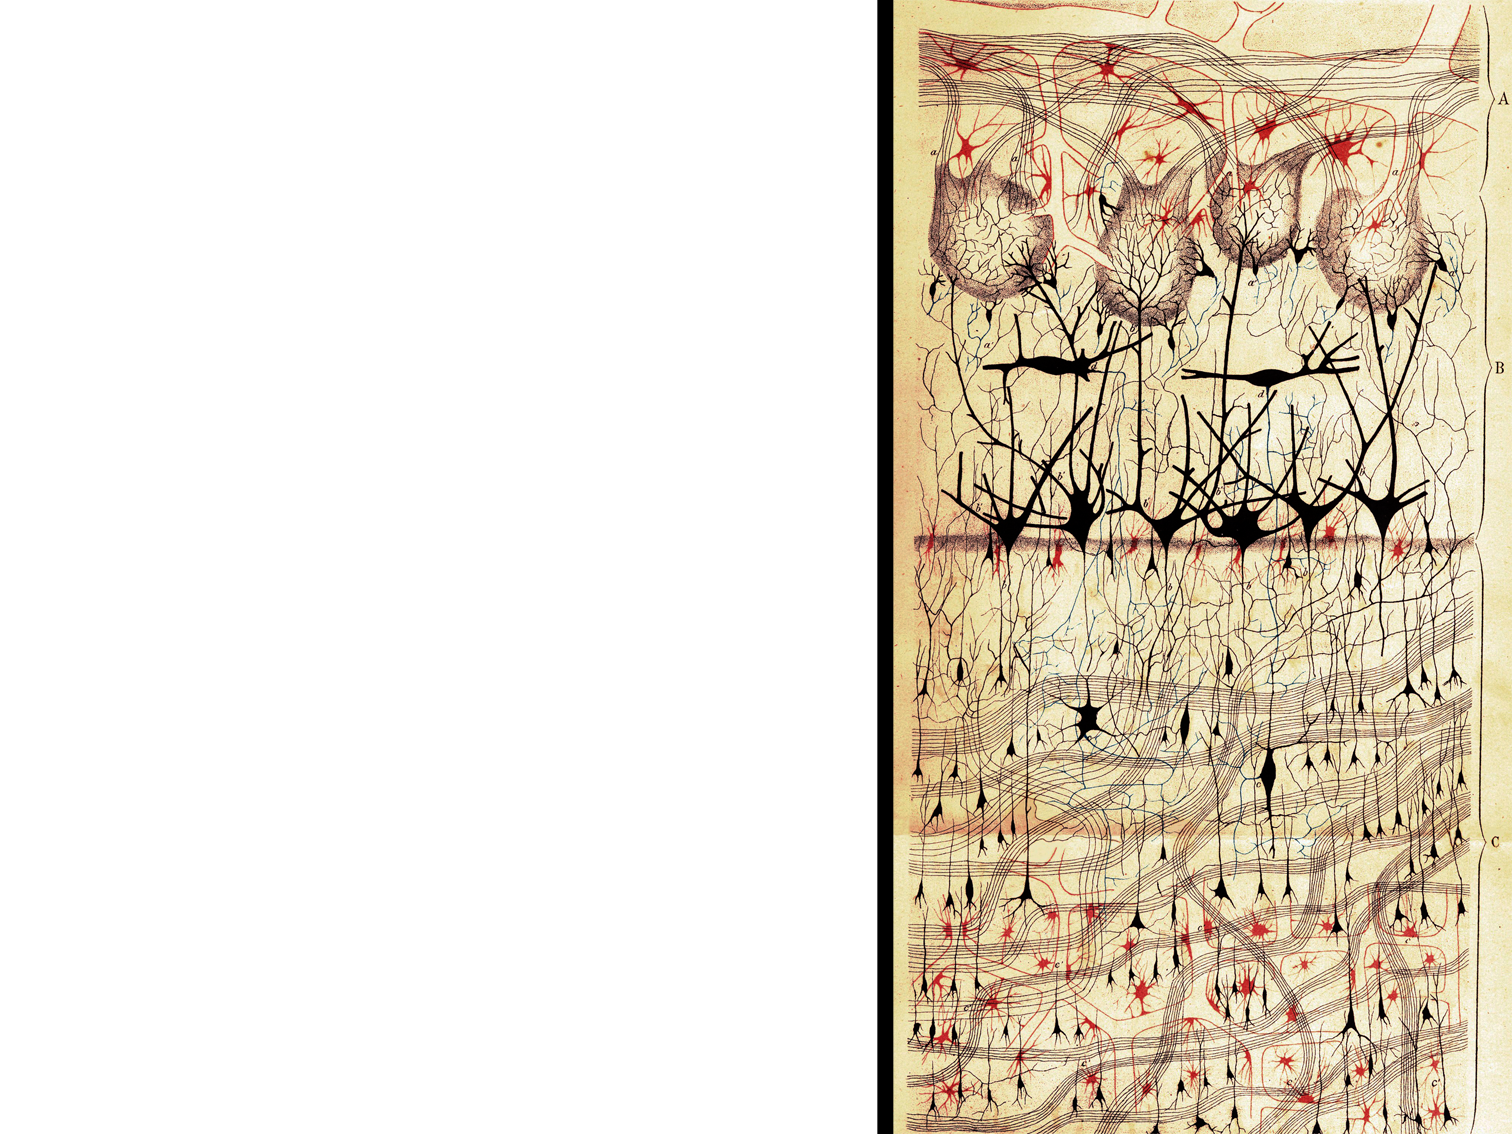
\includegraphics[width=\paperwidth,height=\paperheight]{frontpage_bg}}
	\setbeamertemplate{footline}[default]
		
	{
		\logo{}
		\begin{frame}
			\vspace{2cm}
			\begin{columns}
				\column{2.75in}
				\titlepage
				\vspace{10cm}
				\column{2.0in}
			\end{columns}
		\end{frame}
	}

%-------------------------------------------------------------------
%                          Section 1
%-------------------------------------------------------------------
%
% Set the background for the rest of the slides.
% Insert infoline
\setbeamertemplate{background}{
\includegraphics[width=\paperwidth,height=\paperheight]{slide_bg}}
\setbeamertemplate{footline}[bunsentheme]

\begin{frame}{Sommario}

\tableofcontents

\end{frame}

\section{Principal Component Analysis}

	\subsection{Obiettivi}
	
		\begin{frame}{PCA}
			\begin{itemize}
				\item Trasformazione lineare della matrice dei dati $\mathcal{X}$
				\item Misurazione della variazione delle variabili utilizzando un numero minore di "fattori"
				\item Trasportare il problema in uno spazio \emph{k}-variato (generalmente bi-trivariato)
				\item Semplificazione di visualizzazione e lettura dei dati
			\end{itemize}
		\end{frame}


		\begin{frame}{Esempio}
			\begin{columns}
				\begin{column}{0.5\textwidth}
					\figcen{\columnwidth}{plotTeoria}
				\end{column}
				\begin{column}{0.5\textwidth}
					\begin{itemize}
						\item 40 campioni
						\item 2 variabili
					\end{itemize}
				\end{column}
			\end{columns}			
		\end{frame}

		\begin{frame}{Esempio - 2}
			\figcen{.8\textwidth}{proiezione}
			\begin{itemize}
				\item Nessuna delle due variabili descrive completamente la variabilità dei dati
			\end{itemize}
		\end{frame}

		\begin{frame}{Componenti}
			\figcen{.7\textwidth}{componenti}
			\begin{itemize}
				\item Prendiamo come componenti principali le linee blu
				\item La prima componente spiega la massima percentuale di variabilità rappresentabile in una dimensione
			\end{itemize}
		\end{frame}

		\begin{frame}{Varianza}
			\begin{itemize}
				\item Questa percentuale di variabilità può essere calcolata tramite la varianza
				\item La varianza è un indice della dispersione dei dati lungo una particolare direzione
				\item La varianza è indipendente dal sistema di riferimento
				\item Ruotare gli assi mantiene inalterata la varianza totale
			\end{itemize}
		\end{frame}

		\begin{frame}{Componenti}
			\begin{itemize}
				\item La prima componente cattura quasi tutta la variabilità presente nei dati (99.83\%)
				\item La seconda descrive la rimanente (0.17\%)
				\item Generalizzando, le componenti principali successive spiegano una sempre minore percentuale della variabilità originale
				\item Le ultime componenti principali descrivono principalmente rumore
			\end{itemize}
		\end{frame}

	\subsection{Funzionamento}

		\begin{frame}{Funzionamento}
			\begin{enumerate}
				\item Standardizzazione
				\begin{itemize}
					\item Standardizzare i dati (media = 0, varianza = 1)
					\item Possiamo lavorare con variabili su scale e unità di misure differenti
				\end{itemize}
				\item Calcolo covarianza/correlazione
				\begin{itemize}
					\item Calcoliamo la matrice S di covarianza $$\mathcal{S} = \frac{1}{n-1} \sum_{1}^{n} (x-\mu)(x-\mu)^T$$
					\item Possiamo usare anche la matrice di correlazione
				\end{itemize}
				\item Calcolo autovalori/autovettori 
				\begin{itemize}
					\item $\mathcal{S} \times v = \lambda \times v$
				\end{itemize}
			\end{enumerate}
		\end{frame}

	\begin{frame}{Funzionamento}
		\begin{enumerate}
			\setcounter{enumi}{3}
			\item Scelta delle componenti
			\begin{itemize}
				\item Ordiniamo in maniera decrescente gli autovalori ottenuti
				\item Selezioniamo i primi \emph{k}
				\item Costruiamo $\mathcal{V}$, la matrice dei rispettivi autovettori
			\end{itemize}
			\item Rotazione dei dati
			\begin{itemize}
				\item Moltiplichiamo i dati originali per gli autovettori che indicano le direzioni dei nuovi assi (componenti principali) 
				\item I dati ruotati vengono chiamati \emph{score} $$Sc = \mathcal{X} \times \mathcal{V}$$
			\end{itemize}
		\end{enumerate}
	\end{frame}

\section{Implementazione Python}

	\subsection{Strumenti}

		\begin{frame}{Strumenti utilizzati}
			\begin{itemize}
				\item Linguaggio: Python
				\item Libreria per l'analisi dei dati: \emph{PANDAS}
				\item Dataset: IRIS
			\end{itemize}
		\end{frame}


		\begin{frame}{PANDAS}
			\begin{itemize}
				\item Libreria Python, open source, ad alte prestazioni e con licenza BSD
				\item Strutture dati e strumenti per l'analisi facili da usare (R-like)
				\begin{itemize}
					\item Serie (unidimensionali)
					\item Dataframe (bidimensionali)
				\end{itemize}
				\item Dati organizzati in maniera \emph{relazionale} o \emph{etichettata}
				\item Sponsorizzato da NumFocus
				\begin{columns}
					\begin{column}{.3\textwidth}
						\figcen{\columnwidth}{numFocus}
					\end{column}
					\begin{column}{.7\textwidth}
						\begin{itemize}						
							\item sviluppo continuo, a livello mondiale e sistema di donazioni a supporto
						\end{itemize}						
					\end{column}
				\end{columns}
			\end{itemize}
		\end{frame}

		\begin{frame}{Dataset}
			\begin{columns}
				\begin{column}{.6\textwidth}
					\figcen{\columnwidth}{iris}
				\end{column}
				\begin{column}{.5\textwidth}
					\begin{itemize}
						\item Dataset IRIS
						\item 150 misurazioni di fiori iris 
						\item 3 diverse specie
					\end{itemize}
				\end{column}
			\end{columns}
		\end{frame}

	\subsection{Implementazione}

		\begin{frame}{Caricamento Dataset}
			\codice{16}{25}
			\figcen{.7\textwidth}{tab}
		\end{frame}

		\begin{frame}{Divisione valori}
			\begin{itemize}
				\item Matrice valori numerici $X \in \mathcal{M}^{150x4}$
				\item Vettore specie $y \in \mathcal{M}^{150x1}$
			\end{itemize}
			\codice{30}{32}
		\end{frame}

		\begin{frame}{Analisi descrittiva}
			\codice{37}{56}
		\end{frame}
	
		\begin{frame}{Analisi descrittiva}
			\figcen{.7\textwidth}{isto}
		\end{frame}
	
		\begin{frame}{Analisi descrittiva}
			\begin{itemize}
				\item Valori su scale diverse richiedono standardizzazione
				\item Usiamo la funzione di libreria
			\end{itemize}
			\codice{58}{59}
		\end{frame}
	
		\begin{frame}{Autovalori e autovettori}
			\codice{61}{82}
		\end{frame}
	
		\begin{frame}{Autovalori e autovettori}
		\codice{84}{94}
			\begin{itemize}
				\item In tutti i casi otteniamo la matrice $$\begin{bmatrix}
				0.52237162 & -0.37231836 & -0.72101681 & 0.26199559\\
				-0.26335492 & -0.92555649 & 0.24203288 & -0.12413481\\
				0.58125401 & -0.02109478 & 0.14089226 & -0.80115427\\
				0.56561105 & -0.06541577 & 0.6338014 & 0.52354627\\
				\end{bmatrix}$$
			\end{itemize}
		\end{frame}
	
		\begin{frame}{Selezione componenti}
			\begin{itemize}
				\item Gli autovettori calcolati forniscono solamente la direzione perché sono tutti a norma unitaria
				\item Per scegliere i più interessanti ordiniamo i rispettivi autovalori
			\end{itemize}
			\codice{96}{102}
		\end{frame}

		\begin{frame}{Varianza spiegata}
			\begin{itemize}
				\item Calcoliamo la varianza spiegata dalle singole componenti
				\item Visualizziamo il risultato su un grafico
			\end{itemize}
			\codice{108}{123}
		\end{frame}

		\begin{frame}{Varianza spiegata}
			\figcen{.75\textwidth}{istoVarianza}
		\end{frame}
	
		\begin{frame}{Matrice di proiezione}
			\begin{itemize}
				\item Passiamo da 4 a 2 dimensioni
				\item Estraiamo le prime due componenti dalla matrice degli autovettori
			\end{itemize}
			\codice{125}{127}
			\begin{itemize}
				\item Creiamo la matrice di proiezione $\mathcal{W}$
			\end{itemize}
			$$\mathcal{W} = \begin{bmatrix}
			0.52237162 & -0.37231836\\
			-0.26335492 & -0.92555649\\
			0.58125401 & -0.02109478\\
			0.56561105 & -0.06541577\\
			\end{bmatrix}$$
		\end{frame}

		\begin{frame}{Proiezione}
			\begin{itemize}
				\item Proiettiamo nel nuovo sottospazio $$\mathcal{Y} = \mathcal{X}\times \mathcal{W} \qquad \mathcal{Y} \in \mathcal{M}^{150x2}$$
			\end{itemize}
			\codice{132}{133}
		\end{frame}
		
		\begin{frame}{Risultato}
			\figcen{.8\textwidth}{PCA}
		\end{frame}
		
		\begin{frame}{Post Scriptum}
			\begin{itemize}
				\item Esiste una funzione di libreria che calcola $\mathcal{Y}$ direttamente da $\mathcal{X}$
				\item L'unico parametro da fornire è il numero di componenti che si vogliono prendere in considerazione
			\end{itemize}
			\codice{149}{151}
			\figcen{.3\textwidth}{ok}
		\end{frame}

\section{Caso di studio}

	\subsection{Problema}

		\begin{frame}{Problema}
			\figcen{.5\textwidth}{iot}
			\begin{itemize}
				\item Miliardi di dispositivi informatici connessi in rete nel mondo
				\item Innumerevoli casi di intrusioni malevole in tali sistemi
				\item Il problema della sicurezza delle reti è molto serio
				\item I dati relativi al traffico di rete hanno in genere molte dimensioni
				\item Difficili da visualizzare e analizzare
			\end{itemize}
		\end{frame}
		
		\begin{frame}{Intrusion Detection Systems}
			\figcen{.5\textwidth}{guardia}
		\end{frame}

		\begin{frame}{IDS}
			\begin{itemize}
				\item Gli IDS si dividono in due grandi categorie
				\begin{enumerate}
					\item Signature based
					\begin{itemize}
						\item Riconoscono le \emph{firme} degli attacchi noti
						\item 100\% di successo delle rilevazioni
						\item Riconosco solo attacchi noti
					\end{itemize}
					\item Anomaly based
					\begin{itemize}
						\item Riconoscono un comportamento diverso dal \emph{normale}
						\item Possono riconoscere attacchi nuovi
						\item Possono creare falsi allarmi o non riconoscere qualche attacco
					\end{itemize}
				\end{enumerate}
			\end{itemize}
		\end{frame}

		\begin{frame}{Idea}
			\figcen{.3\textwidth}{idea}
			\begin{itemize}
				\item Possiamo costruire un IDS basato sulla PCA?
				\item Capiamo un po' meglio come funzionano i principali attacchi
			\end{itemize}
		\end{frame}
		
		\begin{frame}{Tipi di attacchi}
			\begin{itemize}
				\item Ci focalizzeremo su due tipi di attacchi
				\begin{enumerate}
					\item Denial of Service (DoS)
					\begin{itemize}
						\item Si cerca di rendere la risorsa sotto attacco troppo occupata (rete) o piena (memoria) per essere utilizzata
					\end{itemize}
						\item Network Probe (NP)
					\begin{itemize}
						\item Scansione sistematica di tutti i dispositivi connessi alla rete e delle loro porte di comunicazione
					\end{itemize}
				\end{enumerate}
			\end{itemize}
		\end{frame}

		\begin{frame}{Attacchi DoS}
			\figcen{.8\textwidth}{dos}
		\end{frame}
		
		\begin{frame}{Attacco SMURF}
			\begin{figure}
				\begin{center}
					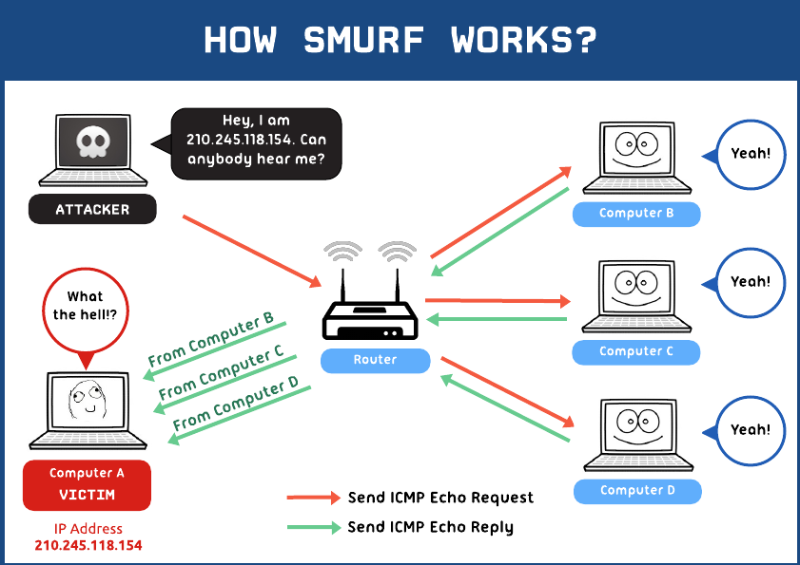
\includegraphics[width=.75\textwidth]{smurf}
				\end{center}
			\end{figure}
		\end{frame}
		
		\begin{frame}{Attacco Neptune}
			\begin{figure}
				\begin{center}
					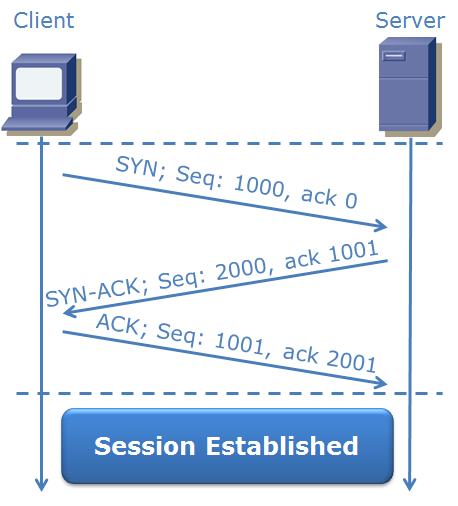
\includegraphics[width=.5\textwidth]{3wayh}
				\end{center}
			\end{figure}
		\end{frame}
	
		\begin{frame}{Attacco Neptune}
			\begin{figure}
				\begin{center}
					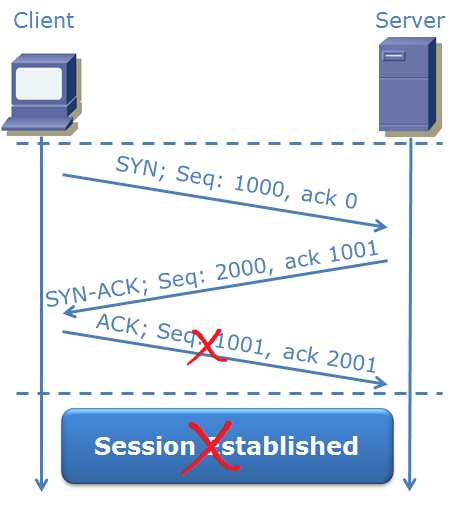
\includegraphics[width=.5\textwidth]{3wayh2}
				\end{center}
			\end{figure}
		\end{frame}
	
		\begin{frame}{Attacco Neptune}
			\begin{figure}
				\begin{center}
					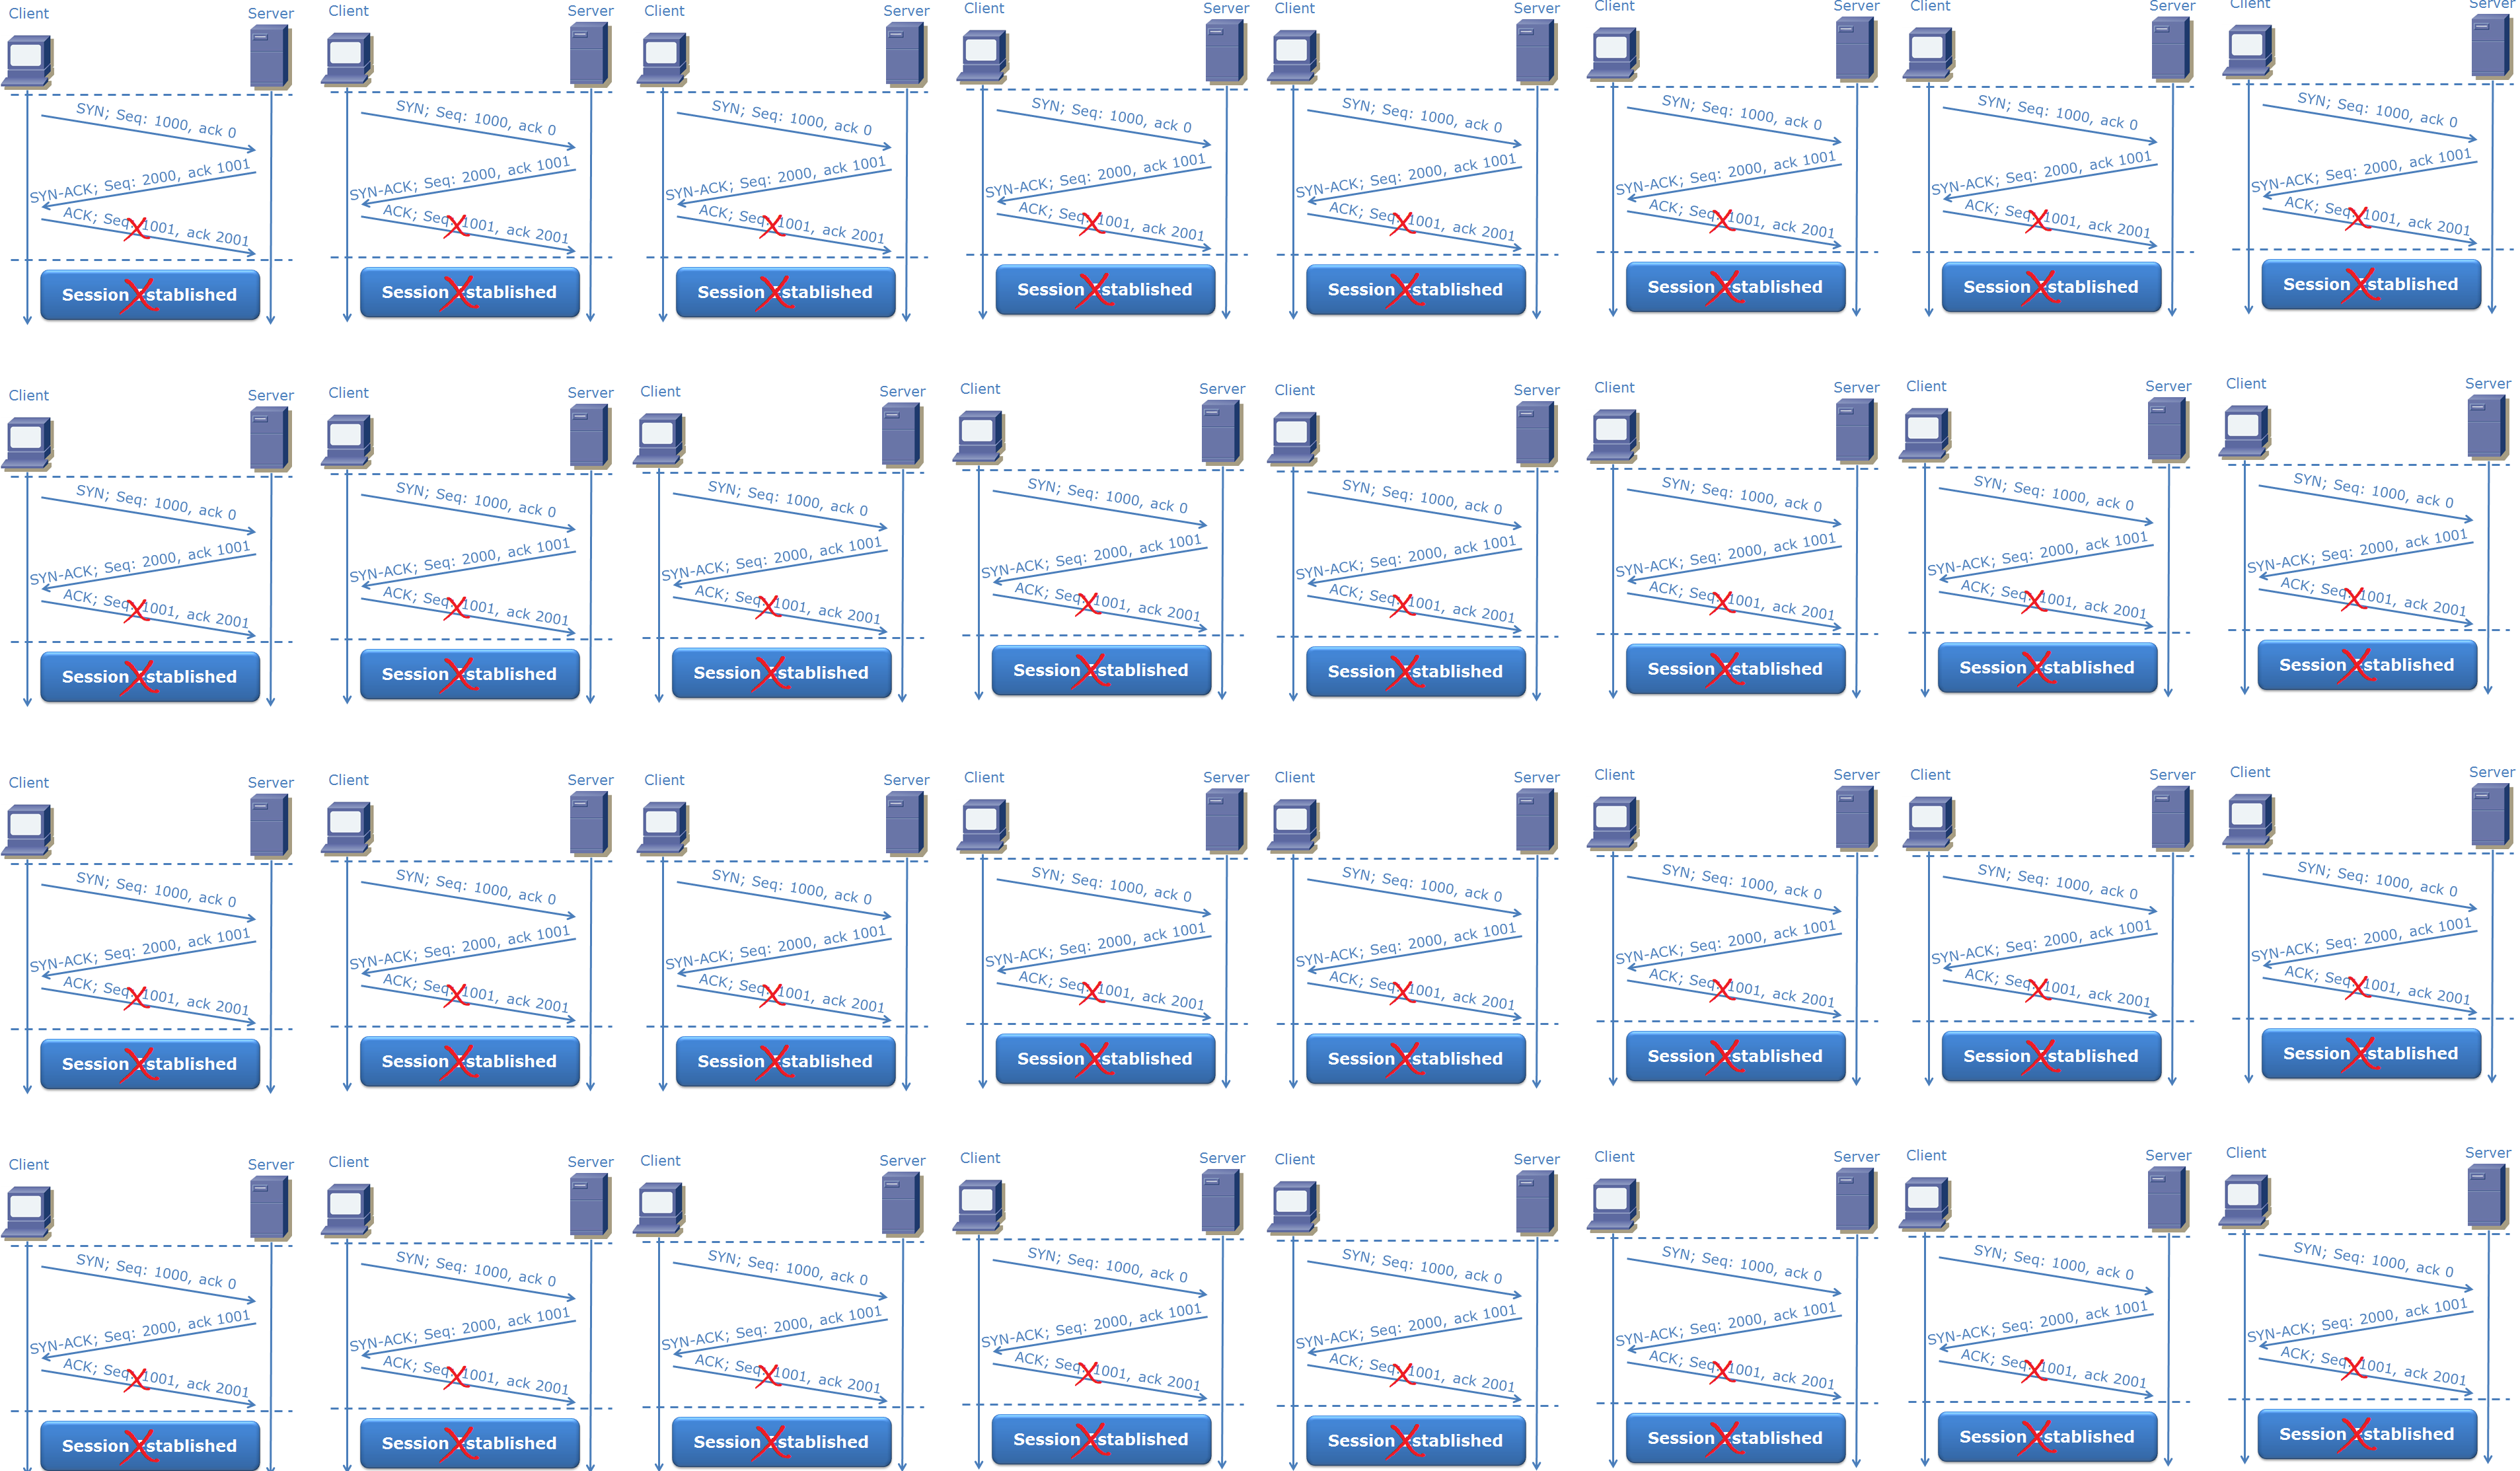
\includegraphics[width=.9\textwidth]{3wayh8}
				\end{center}
			\end{figure}
		\end{frame}

		\begin{frame}{Attacchi NP}
			\begin{itemize}
				\item IPSweep
				\begin{itemize}
					\item Scansione sistematica di tutti gli IP connessi alla rete
				\end{itemize}
				\item PortSweep
				\begin{itemize}
					\item Scansione sistematica di tutte le porte di comunicazione dei sistemi scoperti al passo precedente
				\end{itemize}
			\end{itemize}
		\end{frame}

	\subsection{Esperimento}

		\begin{frame}{Analisi dei dati}
			\begin{itemize}
				\item 1998 DARPA Intrusion Detection Evaluation data sets
				\item Utilizzo della rete in 7 settimane
				\item Presente traffico normale e vari attacchi (tra cui quelli ai quali siamo interessati)
				\item Preprocessing (estrazione delle intestazioni o \emph{header} dei pacchetti di rete)
				\item 12 variabili rilevanti
			\end{itemize}				
		\end{frame}
		
		\begin{frame}{Esperimento}
			\begin{itemize}
				\item Creati 7 dataset (uno per ogni attacco e 3 di traffico normale)
				\item Applicata la PCA ad ognuno di essi per passare da 12 a 2 dimensioni
				\item Le componenti forniranno la direzione della massima varianza
				\item I coefficienti della trasformazione (\emph{loading}) ci indicheranno la malignità/benignità del traffico
			\end{itemize}				
		\end{frame}

	\subsection{Risultati}

		\begin{frame}{Loadings}
			\begin{itemize}
				\item I loadings forniscono informazioni su quanto ogni variabile influisce sulla relativa componente principale (che è una loro combinazione lineare)
				\item Focalizzeremo l'attenzione sulle prime due componenti principali e sui relativi loadings
			\end{itemize}				
		\end{frame}

		\begin{frame}{Loadings}
			\figcen{.6\textwidth}{grafico}		
		\end{frame}

	{ 	
		% all template changes are local to this group.
		\setbeamertemplate{navigation symbols}{}
		\begin{frame}[plain]
			\begin{tikzpicture}[remember picture,overlay]
				\node[at=(current page.center)] {
				
\includegraphics[scale=0.45]{img/All}
				};
			\end{tikzpicture}
		\end{frame}
	}

\end{document}
